\subsubsection{Slicing based hypervisors}
\label{sec:existing-nhv}
In this section we describe the hypervisors using the slicing technique to abstract the physical infrastructure into a virtual network.

\paragraph{FlowVisor}

FlowVisor~\cite{FlowVisor-Sherwood2009} is the first SDN hypervisor implemented.
FlowVisor creates Virtual Networks by slicing the physical infrastructure, and providing each tenant with a set of physical resources (\ie a slice).

Once a tenant has been assigned a slice of physical resources, he will define the flowspace 
corresponding to its traffic.
The flowspace correspond to the set of flow rules that will be used as filters for the tenant's traffic.
Finally, the virtual network presented to the tenant is the set of physical nodes that will match the incoming traffic defined by the flowspace allocated to the tenant.
The tenant will then connect their SDN controller to the slice, enabling them to interact with their virtual network.

% Virtual networks are defined as a set of links between physical SDN switches.
% These links will only match the traffic belonging to the tenant.
% FlowVisor introduce them as flowspace and each flowspace maps a tenant with a physical node and a specific match-action criteria for the traffic.
% For a tenant, the collection of these flowspaces is called a slice and represent their virtual network. 


\begin{figure}[h]
    \centering
    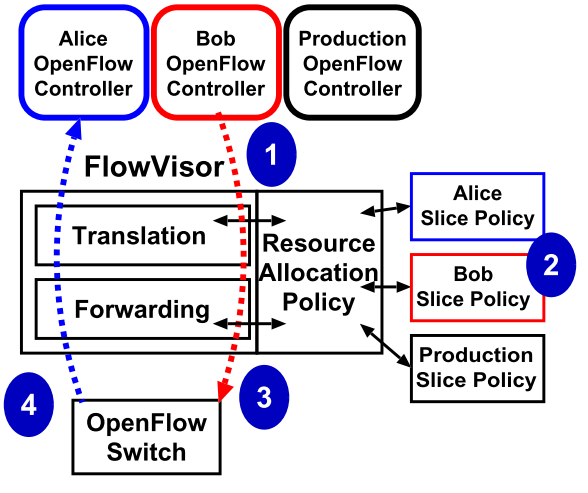
\includegraphics[scale=0.6]{figures/flowvisor-process.png}
    \caption{Message processing in Flowvisor~\cite{FlowVisor-Sherwood2009}}
    \label{fig:flowvisor-process}
\end{figure}

FlowVisor enforces isolation between tenants by acting as a proxy between them and the physical infrastructure, as depicted in Figure~\ref{fig:flowvisor-process}.
FlowVisor abstracts the physical architecture by showing each tenants only the resources that have been allocated to them.
When a tenant wants to deploy an OpenFlow rule (OF rule) on a physical node (1), FlowVisor will intercept it, check the resources allocated to the slice (2) and rewrite match and actions fields so the rule only affects the virtual network and not all the incoming traffic (3).
Similarly, When an OpenFlow message is sent from a physical node to the controller, FlowVisor will intercept the message and forward it only to the tenants whose slice's policy matches the message (4).

Flowvisor provides mechanisms to enforce resource isolation for bandwidth, topology, switch CPU, flowspace, flow entries tables and the southbound interface communications. 
Isolating these resources will prevent a tenant to exceed the amount of resources he has been allocated or prevent a malicious attacker to modify the traffic of another user without authorization.
However, FlowVisor lacks major components related to virtualization, such as arbitrary topologies and virtual network migration.
These aspects have been tackled in several hypervisors based on FlowVisor.

\paragraph{Enhanced FlowVisor}
Enhanced FlowVisor~\cite{EnhancedFV-Min2012} extends FlowVisor by implementing a minimum guaranteed bandwidth feature. It ensures that each tenant of a virtual network will be served with the required amount of bandwidth for all the links in his topology. Information about virtual networks, tenants information etc. are stored in a database. When a new request for a virtual network is received, a potential physical substrate will be mapped to the request. Then Enhanced FlowVisor will query the database to check if each link in the physical substrate satisfies the requested bandwidth of the virtual network. If it cannot, then the request is denied. 
The flowspace used in this solution is based on 3 bits of the VLAN PCP field which restricts the total number of tenants to 8.
Enhanced FlowVisor is based on the NOX controller and uses HP ProCurve switches using the Guaranteed Minimum Bandwidth feature.

\paragraph{Slices Isolator}
Slices Isolator~\cite{SlicesIsolator-El-Azzab2011} is an hypervisor providing resource isolation between slices. A slice is defined as a subdivision of a physical switch, to which flows will be affected. Slices Isolator provides isolation for interfaces, flow processing and memory. Interface isolation consists in either providing a dedicated network interface to a slice or to aggregate incoming traffic to one interface and then distributing the control to the different tenants. Processing isolation defines which flows will be processed using the same rules. Each flow is splitted into two subflows, one is discarded and the other is processed. This helps reducing the size of processing tables but if a poorly designed rule is added it can compromise the expected behavior of the system. Therefore, processing isolation works by determining if the addition of the new rule does not conflict with the previous rules. Determining potential conflicts between existing rules and the next rule to be added works as follows: if the filters used by the new flow rule does not overlap with existing filters, then there is no conflict.
If there is overlap, there is a conflict if and only if the overlap between the new flow rule and the existing one is not on the discard subflow but on the processed subflow.Finally, memory isolation is implemented with queuing algorithms for the traffic, ensuring a slice does not overload its allocated resources. 

\textbf{Conclusion:} Overall, network hypervisors using slicing have not been designed to support the migration feature but are oriented toward providing resource isolation between slices. Because the set of network slices is limited by the physical infrastructure, it will not always be possible to find another slice that will match the original topology of the virtual network.

\subsubsection{API based hypervisors}
API based hypervisors are using specific API to manage virtual networks and to allow tenants to interact with them.

\paragraph{Network Hypervisor}
The Network Hypervisor~\cite{NetworkHypervisor-Huang2013} aims at providing a unified virtualization over multi-domains SDN infrastructures. 
% Authors present a vision of the future of SDN network and how infrastructure providers, services resellers and users would work to provide a seamless virtualization service that would alleviate the maintenance operations burden from the tenants.
The ultimate goal of the Network Hypervisor is to enable HyperNets~\cite{HyperNet-Huang2013a}. HyperNets are envisioned as a sort of final form for SDN services. A user may request a virtual network to serve specific needs (\eg Video Streaming) and connect specific clients together.
The HyperNet should be able to automatically determine what are the physical resources that should be allocated in terms of positioning, computational power etc. In addition to this, HyperNets should provide routing procedures specifically design for the requested service (\ie prioritize video traffic over less relevant traffic).
In order to provide the support of said HyperNets, the Network Hypervisor provides API functions. These functions includes network discovery so they can allocate suitable physical resources close the HyperNet users as well as design a suitable topology to interconnect all participants.
Moreover, they implement a dynamic join/leave feature, where users will be allowed to connect to a SDN virtual network without being directly connected to one. The use of IP tunneling solves such connectivity issues.
Aside from these high level API functions, the role of the Network Hypervisor is to concatenate the different network resources connected to it.
This hypervisor has been implemented to work on top of the ProtoGENI~\cite{protoGENI} infrastructure.

\paragraph{Compositional Hypervisor}
The aim of Compositional Hypervisor~\cite{CompositionalHypervisor-Jin2014} is to provide an homogeneous layer between SDN controllers and tenants application.
Each application is designed to work with a specific SDN controller and is based on a specific programming language. Therefore, it is next to impossible for a tenant to concurrently run different applications from different environments because they will conflict with each other. Compositional Hypervisor sits between the physical infrastructure and the SDN applications used by tenants.
Each application generates a set of flow rules, which is referred to as a policy.
Upon receiving each generated policy, the tenant is then able to combine them together using a specific arithmetic.
This arithmetic allows to have policies being enforced either in parallel or sequentially. 
In Figure~\ref{fig:compositional-hyp}, a load balancing application co exist with a routing and a monitoring application. The arithmetic shows that the load balancing rules should process the traffic first, and then the routing and monitoring applications will see their flow rules combined into a unique treatment.
This composition simplifies the OF rules deployed in each switch by providing a unique list of prioritized OF rules. When one of the policies is update, the hypervisor will recompute the updated policy depending on whether a rule has been added/removed/modified.

\begin{figure}[ht]
    \centering
    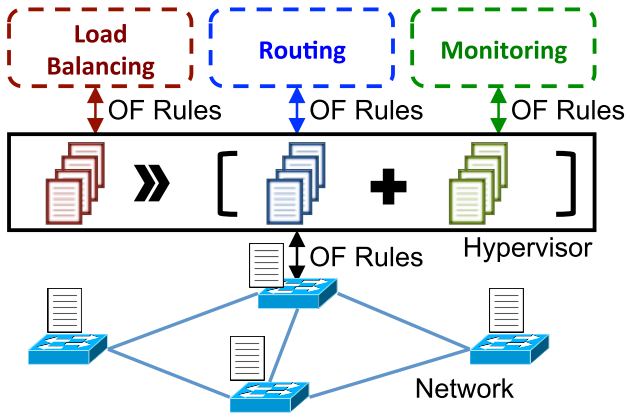
\includegraphics[scale=0.7]{figures/compositional-structure.png}
    \caption{Flow rules arithmetic from Compositional Hypervisor~\cite{CompositionalHypervisor-Jin2014}}
    \label{fig:compositional-hyp}
\end{figure}

From an architectural point of view, users are not presented with their own virtual network that they will be able to modify at will, but instead the manipulation of the physicak infrastructure is abstracted to implement an efficient OF rules deployment abd ti allow the coexistence of heterogeneous solution.


\subsubsection{Mapping based hypervisors without migration}
The hypervisors presented in this section maintain a mapping between the virtual network they disclose to the tenant and the physical resources used to support the corresponding virtual network but do not support the migration of virtual networks.

\paragraph{ADVisor}
ADVisor~\cite{ADVisor-Salvadori2012} is based on FlowVisor and tackles two design issues introduced with FlowVisor.
The first contribution is the implementation of arbitrary virtual topologies.
Instead of slicing physical resources and presenting them to the tenants, 
The virtualization completely decouples the abstract view of the virtual network from the physical resources supporting it.
A virtual link between two virtual nodes might in fact be composed of several physical links. The role of ADVisor is to hide these intermediate nodes from the tenant.

The second contribution of ADVisor consists in the sharing of the flowspace proposed by FlowVisor.
Originally, the definition of a flowspace would restrict the manipulation of a certain type of traffic (\eg port 80, source MAC address) to only one tenant.
Giving access of one flowspace to two different tenants would break the isolation and allow one to control and alter the traffic of the other.
The same limitations come regarding the address space available to tenants.
ADVisor alleviate this limitation by defining a set of identifiers that will be allocated to each tenant. These identifiers are referred to as "flowspace`` but they do not exactly hold the same meaning as defined by FlowVisor~\cite{FlowVisor-Sherwood2009}. Indeed, each tenant has access to the whole flowspace (\ie the whole header fields) except for the few bits reserved by ADVisor to store the necessary identifiers.

\begin{figure}[h]
    \centering
    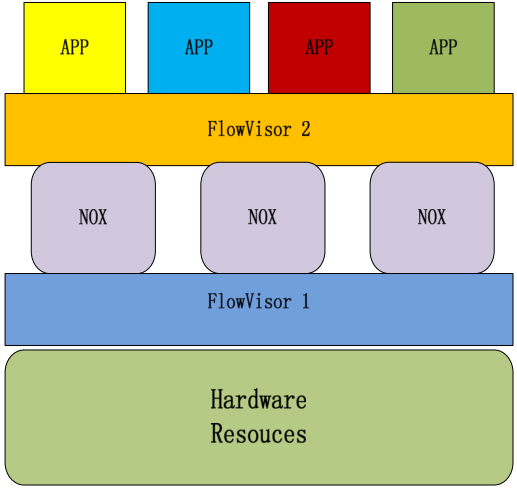
\includegraphics[scale=0.6]{figures/double_fv.png}
    \caption{Architecture of Double FlowVisor}
    \label{fig:double-fv}
\end{figure}

\paragraph{Double FlowVisor}
Double FlowVisor~\cite{DoubleFV-Yin2013} combines two instances of FlowVisor to virtualize a multi-domain network and provide a unified view of the virtual network, as presented in Figure~\ref{fig:double-fv}. The first instance of FlowVisor (FlowVisor 1) is used to hide the heterogeneity of the different network domains. These domains are connected together and are abstracted and a NOX controller~\cite{nox-gude2008} is connected to FlowVisor.
Then, the second FlowVisor  (FlowVisor 2) instance will connect NOX with the tenants' applications. This instance maintains the embedding between virtual resources and the physical substrate, and translates commands sent by the tenant into commands deployed in the physical infrastructure. In addition to that, the second FlowVisor instance is in charge to tag each flow with an identifier related to the tenant.

\begin{figure}[h]
    \centering
    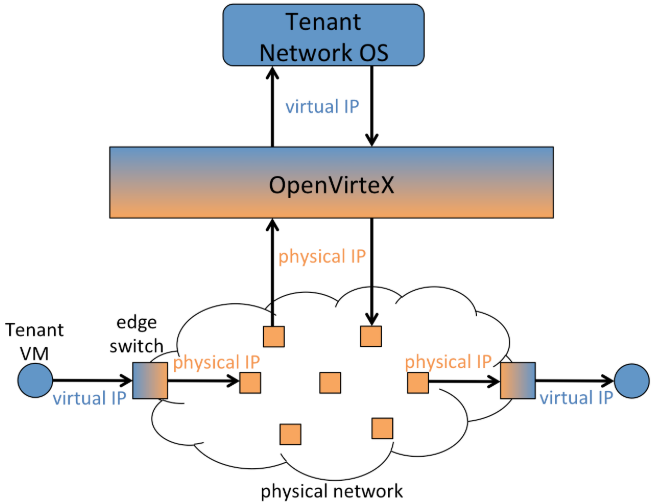
\includegraphics[scale=0.7]{figures/openvirtex.png}
    \caption{Identifier translation at edge switches in OpenVirteX~\cite{OpenVirteX-Al-Shabibi2014}}
    \label{fig:openvirtex}
\end{figure}

\paragraph{OpenVirteX}
OpenVirteX~\cite{OpenVirteX-Al-Shabibi2014} (OVX) is a network hypervisor based on the same design as FlowVisor~\cite{FlowVisor-Sherwood2009}. OVX serves as a proxy between the tenants' controllers and the underlying physical infrastructure. OVX provides both full virtual topology abstraction and full address space abstraction. 

When a tenant requests a virtual network, he describes the different resources, nodes and links he needs.
Then OVX will determine the adequate physical substrate to embed the virtual network.
The virtual/physical resources mapping is stored by OVX and is used to present the virtual topology to the controller.
While FlowVisor will hide messages to unintended recipients, OVX intercept LLDP packets used for topology discovery. Everytime a LLDP message arrives at a virtual switch, OVX uses the mapping to determine the virtual node at the other end of the virtual link. A LLDP response is forged by OVX with matching information and forwards it to the corresponding tenant's controller.

OVX enables tenants to use the full address space by assigning an identifier to each tenant and then combining it with a unique identifier for each host. Figure~\ref{fig:openvirtex} depicts the two cases where the identifier translation is performed. In the first case, when the tenant Network Operating System wants to deploy flow rules, he will specify his own virtual identifiers. OpenVirteX will intercept the flow rules, translate the virtual IP addresses into the corresponding physical ones. The second case is when traffic goes through an edge switch of the network, the switch is in charge of translating the IP headers back into the flowspace used by the VM.

\paragraph{SR-PVX}
SR-PVX~\cite{PVX-Li2017} is the first network hypervisor supporting Protocol Oblivious Forwarding~\cite{pof-song2013} (POF). POF is an extension of the concept set up by OpenFlow~\cite{Openflow-McKeown2008}, where developers may implement new protocols without the constraints of the OpenFlow protocol.
SR-PVX provides two main features, the improved programmability of the POF paradigm and a reduced resource consumption to implement network virtualization.

The programmability proposed by POF is to replace protocol specific headers by a set of \textit{\{offset,length\}} tuples. This way, developers will be able to specify their own data structures to be processed by the switch. This allows to use Source Routing (SR) where routing instructions are encapsulated inside the packet to transmit across the network.
SR-PVX decouples the virtual topologies from the underlying physical infrastructures.
Upon receiving a virtual network request, a Network Embedder will determine the optimal physical substrate. Then the hypervisor will generate the related specific forwarding instructions and deploy them only inside the physical switches used to embed virtual nodes. Every other physical switch used to connect two virtual nodes is hidden from the tenant's view and is abstracted as part of the virtual link.

In SR-PVX authors outline the physical limitations encountered by physical switches. If one wants to host a realistic use case of datacenter usage, with a high number of tenants, where users often interacts with the system to configure their networking needs or where regular changes occur in the infrastructure due to physical failure or VM relocation, traditional network hypervisors will quickly exceed the capacities of the network equipments. SR paradigm is leveraged to tackle this issue. At each physical node, embedding a virtual switch are installed encapsulation rules toward the next virtual switch. Between them may sit several switches with no rules deployed. Instead, they will treat incoming traffic by decapsulating the next available header indicating to which port the packet must be sent. By reducing the number of switches on which the rules must be installed, SR-PVX greatly improves the resource consumption of SDN virtualization. Authors propose in~\cite{pvflow-Li2018} a flowtable virtualization mechanism that improves the work done with the design of SR-PVX.


\paragraph{WhiteVisor}
WhiteVisor~\cite{whitevisor-Yu2019} is designed to support SDN-based virtualization on white box switches.
White box switches are networking elements that do not natively embark any operating system and simply provide network forwarding functions that will be used by the operating system.  
The main challenge of using these switches id that they provide a specific set of instructions and flowtables depending to process packets. Moreover, L2 and L3 routing is not performed on the same flowtables and associated pipelines.
WhiteVisor is based on two main components, a virtual to physical pipeline converter as well as a storage component.
The pipeline converter translates a virtual pipeline by decomposing it and installing in the different flowtables of the white box switch. WhiteVisor implements both Layer 2 and Layer 3 routing and details the different mechanisms associated to each routing scheme. Authors also highlights technical constraints of white box switching related to the ordering of flow processing and header matching. The storage component is used to keep a mapping of the physical and virtual pipelines and notifies tenants when a pipeline is removed. 


\paragraph{ONVisor}
ONVisor~\cite{ONVisor-Han2018} is a network hypervisor based on the ONOS~\cite{onos-Berde2014a} controller.
It has been designed along three main ideas, a distributed hypervisor to provide flexibility and scalability, an abstraction of the heterogeneous hardware implementation and finally VN federation to allow different virtual networks of a same tenant to interact together.
ONVisor implements network virtualization by extending how ONOS interacts with the physical infrastructure.
ONVisor implements two new components, the \textit{Virtual Provider} and the \textit{Virtual Manager}.
The \textit{Virtual Manager} provides tenants with service interfaces, similarly ONOS does. Tenants will be able to interact with their VN through this component.
The \textit{Virtual Provider} will in turn receive the commands sent from the \textit{Virtual Manager} and translate them so they can be deployed in the physical infrastructure. This component will also receive networking events and changes coming from the network and will translate them and forward them to the tenants' applications.

\subsubsection{Mapping based hypervisors supporting the migration}
The hypervisors presented in this section abstract the physical resources behind a mapping with the virtual network presented to the tenant. In opposition to the previous section, these hypervisors provide a form of network migration. 

\paragraph{VeRTIGO}
VeRTIGO~\cite{VeRTIGO-Corin2012a} is an extension of the work done with ADVisor and offers two different types of virtual networks.
Either the tenant will have the full control over the virtual network (including traffic engineering techniques etc.) or he will be presented with a single node and leave the handling of network operations to the service provider.
This abstract view is often called ``Big Switch Abstraction".
It provides networking to a tenant who is not interested in handling network operations himself.

VeRTIGO implements virtual network migration using a component called VT Planner. The VT Planner consists in a set of precached virtual topologies that will be deployed in case of link failure. In case of link congestion of physical failure, the VT Planner will migrate the virtual network by deploying the configuration rules into the new network equipments.

\paragraph{CoVisor}
CoVisor~\cite{CoVisor-Jin2015} extends Compositional Hypervisor~\cite{CompositionalHypervisor-Jin2014} by making two significant contributions.
The first one is a novel policy combination algorithm that will focus on the performance of the policy deployment in terms of packets send and computation time.
CoVisor exploits the policies being composed to generate specific data structures that will serve as rules indexes.
Regrouping composed policies based on the common fields they affect reduces the number of rules pair considered at compilation time.
Similarly, they correlate common attributes between policies to serve as indexes for storage. Determining the intersection of the matching fields for two policies determines the index storage for the composed policy.
This algorithm also support the case where a single physical node spans multiple virtual switches.

The second contribution is related to the view provided by the hypervisor to each application.
CoVisor present an abstract view of the topology based on the needs of the application, thus enhancing the security of the infrastructure by only granting rights for the requested usage. 
For instance, a firewall may only see the infrastructure as a big switch since the incoming traffic should be dropped at the ingress point of the network.
Similarly, a routing application will require full access to the network to determine the optimal routing paths.
CoVisor also limits the actions available to each application using a fine-grained control over the capacities of each controller.
For example, a MAC learner application should only match packets based on MAC addresses, or a firewall should only be able to accept or drop packets, and not to modify them.
By design CoVisor implements two fail-over mechanisms regarding controller failures and switch failures.
Controller failure is handled by introducing a third operator in the policy composition, namely the override operator. This operator specifies which policy to apply if another fails.
In case a physical switch fails, CoVisor notifies each application impacted by the failure and redeploys required OF rules elsewhere in the network when possible.


\paragraph{FlowN}
FlowN~\cite{FlowN-Drutskoy2012} is a network hypervisor designed to provide a full abstraction of the physical infrastructure and to propose a container-based application virtualization system. 
The hypervisor serves each tenant with a custom virtual topology. The virtual topology requires a specific number of nodes and links but FlowN also implements bandwidth reservation as well as maximum latency per link. The decoupling of the virtual network from the physical substrate removes the burden of network maintenance from the tenant and leaves it to the service provider. In case of a switch or link failure, FlowN will migrate the virtual node on a new physical switch without having to notify the impacted tenants.

The virtualization of the control layer places FlowN between tenants' applications and the physical infrastructure. When a SDN application makes a function call, FlowN will intercept it and translate it to preserve the mapping between virtual address space and the physical address space. Since FlowN is based on the NOX~\cite{nox-gude2008} SDN controller, tenants application are limited by the capacities of this controller. 
The design of an API between applications and hypervisor is in opposition to the concept of FlowVisor~\cite{FlowVisor-Sherwood2009} where tenants directly interact with the physical nodes and FlowVisor only restrict and translate OF rules to respect the isolation requirements of the virtualization.

FlowN also offers the full abstraction of the address space for the tenants.
Each tenant will be able to use all the header fields, and FlowN will maintain through the use of a database the mapping between the physical node address space and the virtual one. FlowN uses encapsulation at the ingress point to determine to which tenant the packet must be forwarded. Encapsulation is based on VLAN tagging, in a similar fashion to Nicira~\cite{nicira}.   
FlowN leverages the capabilities of databases to improve the performance of the mapping.



\paragraph{AutoSlice}
AutoSlice~\cite{AutoSlice-Bozakov2012} is designed to tackle the scalability issues of a distributed hypervisor, and optimize resource consumption of physical switches to overcome specific limitations.
In~\cite{AutoSlice-Bozakov2012} authors present the basis of the AutoSlice hypervisor.
Each physical SDN infrastructure is managed by its own controller proxy (CPX).
Each CPX is in charge of accessing corresponding physical switches and translating OF rules from the virtual flowspace to the physical one.
AutoSlice instantiate virtual networks over several SDN domain and each CPX deploys the corresponding OF rules in their infrastructure.
Each CPX is in charge of migrating virtual resources within their own domain.
AutoSlice overcomes the physical limitations of Openflow switches by delegating part of OF rules storage to Auxiliary Software Datapaths (ASD).
These ASD are software switches running on ommodity servers and therefore have the sufficient resources to store all the possible OF rules.
AutoSlice uses a statistical distribution law to determine that low volume flows will generate most of the OF rules and store them in ASD. In opposition, the biggest volume flows use a minimum of OF rules and deploy them inside the physical switches.
In~\cite{AutoSlice2-Bozakov2014} authors go into more details about several design requirements they have expressed. They extend the notion of isolation between tenants by introducing a set of identifiers to prevent overlapping OF rules installed by different tenants.
The isolation of flow tables is ensured by adding a \textit{Virtual Table Identifier} thus sharing the physical flow table among the different tenants.
Similarly, all packets are marked with a \textit{Packet Identifier} so it can be mapped with th \textit{Virtual Table Identifier} and determine how the packet should be processed.
Authors also propose virtual network migration techniques based on information duplication, and highlight the potential excessive usage of flow table resources.
There is no evaluation provided in both~\cite{AutoSlice-Bozakov2012} and~\cite{AutoSlice2-Bozakov2014}.

\paragraph{NVP}
The Network Virtualization Platform~\cite{NVP-Koponen2014} (NVP) proposes a network hypervisor for multi-tenants datacenters. Instead of focusing on virtualizing the physical network of the data center, NVP provides a virtual network on top of OpenvSwitches~\cite{openvswitch} deployed in each VMWare Hypervisor. Those virtual switches are then interconnected using tunnels for end-to-end communication. The physical network is simply used as traditional networking and is assumed to possess standard capacities.
The paper makes several contributions: the implementation of the logical networks based on OpenvSwitch (OVS), the creation of a Domain Specific Language (DSL) to declare the connectivity between hypervisors, switches etc. and tackle scalability and availability issues encountered by NVP.

The logical networks proposed to a tenant in NVP consist in creating a virtual slice inside each OVS which in global sets a logical pipeline between the different VMs pertaining to the tenant.
Each VM hypervisor hosting VMs belonging to a specific tenant will instantiate a \textit{logical datapath} inside its own OVS. 
Then, for each pair of logical datapaths that have been created NVP will create a tunnel between them.
Each time an incoming packet goes through an ingress port of the hypervisor the packet will be redirected to the correct logical datapath then transmitted to the logical datapath corresponding to the destination VM.
The tenant can configure these datapaths with regard to switching, routing and security matters, similarly to traditional networking elements.
The isolation between tenants is ensured by affecting unique identifiers to each logical datapath, preventing unauthorized access to the tenant's traffic.
NVP implements failover mechanisms of physical networking elements as well as controllers by running backup nodes with similar function that will be used in case of a failure.

NVP introduces \textit{nlog}, the DSL proposed in NVP is used tackle the computational challenge of keeping up with the evolution of the forwarding state inside the logical datapaths. Changes in the forwarding state include entries and departures of tenants inside the infrastructure, migration of the different VMs, reconfiguration of logical datapaths by the tenants. \textit{nlog} presents an logical abstraction that decouples the concrete forwarding state and rules from the logic described by NVP. Note that \textit{nlog} is not used by tenants but by NVP when instantiating logical datapaths for tenants.
Tenants are provided an API to interact with NVP.
Using \textit{nlog} to describe the state of the logical abstractions enables an incremental computing of the forwarding state that is resource efficient compared to a naive implementation where any change requires the full recomputation of the forwarding state.

Scalability inside NVP is ensured by distributing computation over several logical controllers and physical controllers. Logical controllers compute the flow and tunnels corresponding to datapaths. Physical controllers are in charge of the communication with the different service nodes, gateways and hypervisors.
Sharding mechanisms are responsible for the availability of the different nodes inside the infrastructure. A sharding coordinator will monitor the signals sent by the different nodes and will promote a node to the master role if the current master fails.

The evaluation of NVP focuses on two things, the time and resources required to setup NVP in different scenarios and the available throughput based on which tunneling mechanism is used by NVP. Theses results are then followed by a serie of reflexions based on the experience gained after the implementation of NVP and how design challenges have been tackled.

\begin{figure}
    \centering
    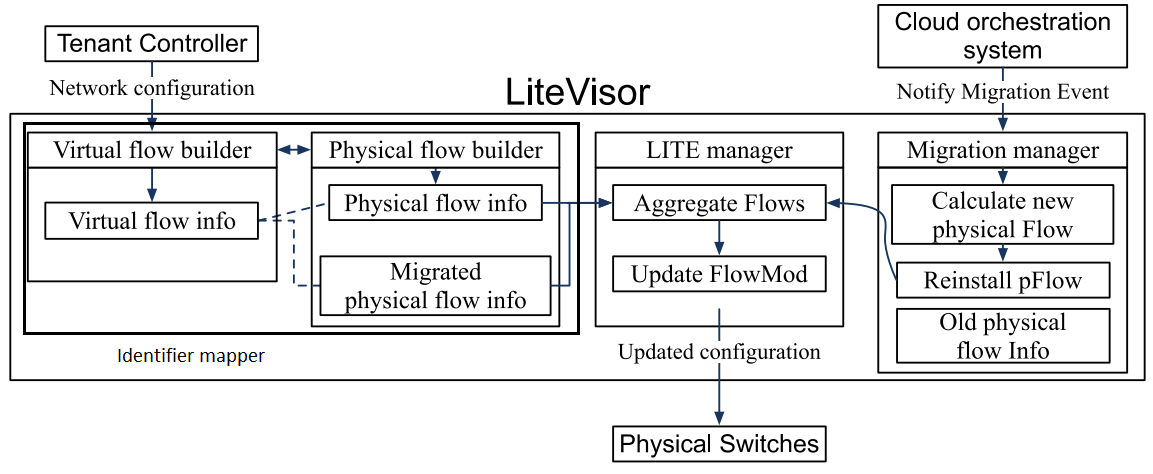
\includegraphics[scale=0.5]{figures/litevisor.png}
    \caption{LiteVisor architecture~\cite{Litevisor-Yang2018}}
    \label{fig:litevisor}
\end{figure}

\paragraph{LiteVisor}
LiteVisor~\cite{Litevisor-Yang2018} is a SDN hypervisor supporting network reconfiguration for VM migration.
Author outline the previous work on flow aggregation to reduce the consumption of switch resources as well as the performance-sensitive context of datacenters and the limitations of existing encapsulation techniques.
LiteVisor is divided in three components illustrated in Figure~\ref{fig:litevisor}. The first one ensures the mapping between virtual and physical identifiers and translates messages sent between tenants and the controller.
The second component is the LITE manager, responsible for aggregating flows sent by the tenant's controller, as well as deploying them on the physical switches. 
The last component is the migration manager. When a VM is migrated, the cloud orchestration system notifies the migration manager about the new location of the VM. The manager then computes a new physical flow that will be transmitted to the LITE manager, which in turns decides if it can be aggregated with an existing flows or deploys the according configuration rules in the physical infrastructure.

